\section{MATLAB}

\subsection*{Vectors and Matrixes}


\begin{frame}[fragile]
  \frametitle{Vectors and Matrixes}

Define vectors:

\begin{lstlisting}
v = [1;2;3;4];     % a vertical vector
h = [1 2 3 4];     % a horizontal vector
M = [[1;2] [3;4]]; % a 2x2 Matrix
s = 1:4;           % the same as h
\end{lstlisting}

Calculate with vectors:
\begin{lstlisting}
u = 5 * v    % multiply vectors by a scalar
w = u - v    % subtract two vectors
x = u .* v   % componentwise multiplication
y = [u v]    % concatenation of vectors
\end{lstlisting}

Example: polar to Euclidean coordinates
\begin{lstlisting}
x = sin(theta) .* cos(rho)
y = sin(theta) .* sin(rho)
\end{lstlisting}

\end{frame}

\subsection*{Indexing of Vectors}

\begin{frame}[fragile]
  \frametitle{Vectors}


Indexing by numbers:

\begin{lstlisting}
v(1)     % the first element
v(2:end) % the last three elements
M(2,1)   % the bottom left element
M(:,2)   % the second column
\end{lstlisting}

Indexing by conditions:

\begin{lstlisting}
v( v > 1 )   % all elements that are larger then 1
v( u == v)   % all elements where u and v coincides
\end{lstlisting}

Changing elements

\begin{lstlisting}
v(1:3) = 1       % set the first three elements to 1
v( v == 0 ) = [] % remove all zeros
\end{lstlisting}

\end{frame}

\subsection*{Working with Data}


\begin{frame}[fragile]
  \frametitle{A First Script}

Load raw pole figure data stored in a column formated ascii file and plot the
data as colorcoded circles.

\begin{lstlisting}
uiimport([mtexDataPath '/juelich/104.hem']);

theta = data(:,1);     % first row is polar angle
rho = data(:,2);       % second row is azimuth angle
intensity = data(:,3); % third row is intensity

scatter(rho,theta,50,intensity,'filled') % plot data

\end{lstlisting}

\center{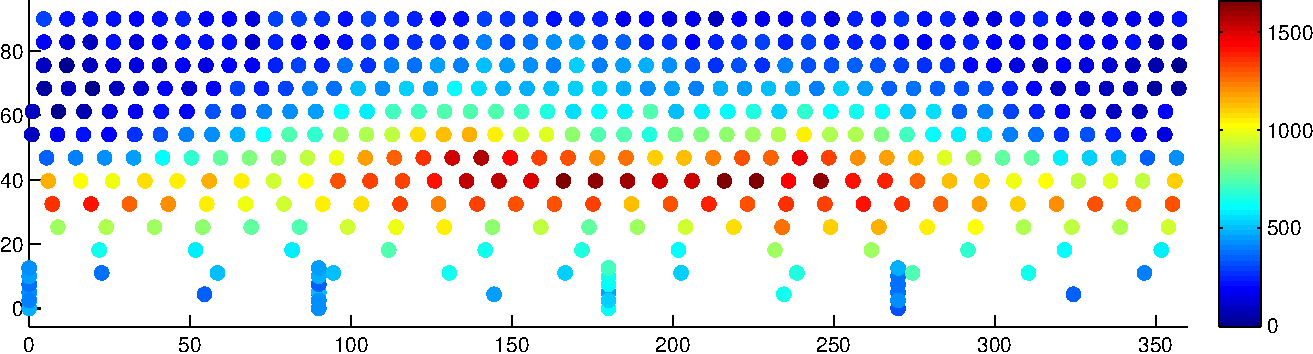
\includegraphics[width=10cm]{pic/scatter}}

\end{frame}


\subsection*{Exercises}

\begin{frame}

  \begin{Exercise}
    \begin{enumerate}[a)]
      \item  Construct a vector \textbf{e} of all even numbers between 10 to 30.
      \item  Construct a vector \textbf{s} of the first 11 sqare numbers.
      \item  Set in \textbf{s} all values to 0 where \textbf{e} $>$ \textbf{s}!
    \end{enumerate}
  \end{Exercise}

  \begin{Exercise}
    \begin{enumerate}[a)]
    \item Load the file \texttt{data/juelich/104.hem} and plot the data as a
      scatter plot!
    \item Determin the minimum, maximum and mean
      intensity of the data!
    \item Plot a histogram of the intensities.
    \item Transform the data into cartesian coordinates and plot them!
    \item Remove all negative values from the data and plot them!
    \end{enumerate}
  \end{Exercise}
\end{frame}



%%% Local Variables:
%%% mode: latex
%%% TeX-master: "main"
%%% End:
